\subsection{Composition Concepts}

A major challenge during the development of a \ms{} application is to achieve
loose coupling according to the IDEAL tenet. It is the goal of loose coupling to
reduce dependencies among services. It has to be noticed that the coupling
between services can never be zero. Without any coupling the application cannot
function as a whole. MicroNet offers several basic concepts to reduce service
coupling while at the same time preserving reasonable development comfort. These
concepts are discussed in this section.

\subsubsection{Dependency Abstraction}

Dependency abstraction is a concept used to reduce the number of dependencies
that \mss{} must explicitly add to the Java classpath to access the core
functionality networking, persistence, and serialization.

According to the dependency abstraction concept external libraries are wrapped
within the core framework to offer standard access to the underlying dependency.
\mss{} can use the MicroNet wrapper libraries instead of directly using the
dependencies. This allows for exchangeability of the dependencies
without touching any \ms{}. MicroNet integrates dependent libraries
into the wrapper libraries by the use of Maven which allows a very flexible
dependency chain. \autoref{fig:dependency_abstraction} shows which libraries are
abstracted by which framework component.

\begin{figure}
	\centering
	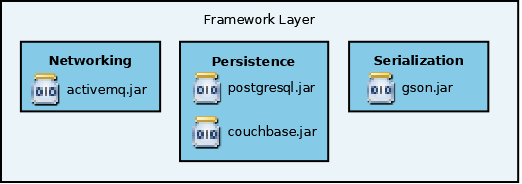
\includegraphics[width=10cm]{images/architecture/DependencyAbstraction}
	\caption{Dependency Abstraction in the MicroNet core framework.}
	\label{fig:dependency_abstraction}
\end{figure}

It has to be mentioned that the dependency abstraction layer is a dependency in
itself which therefore increases service coupling. But since the abstraction
layer unifies dependency access it helps to respect the \glsreset{dry}\gls{dry}
principle and therefore increases the overall cohesion of the application. 

Since the MicroNet adaption layer is realized using Java wrapper libraries,
this approach works very well for all Java \mss{} but services which are not
implemented in Java have to use the dependencies directly.

\subsubsection{Shared Model}
\label{subsub:shared_model}

The general design of incorporating a game model into a \mn{} application is
inspired by the design of modern game engines like Unity3D or UnrealEngine 4.
What these engines have in common is a graph to store the game state e.g. all
objects, levels, players, etc. This concept of game data organization will be
referred to as the game graph. Two examples of game graphs are shown in
\autoref{fig:scenegraph}.

\begin{figure}
  \centering
  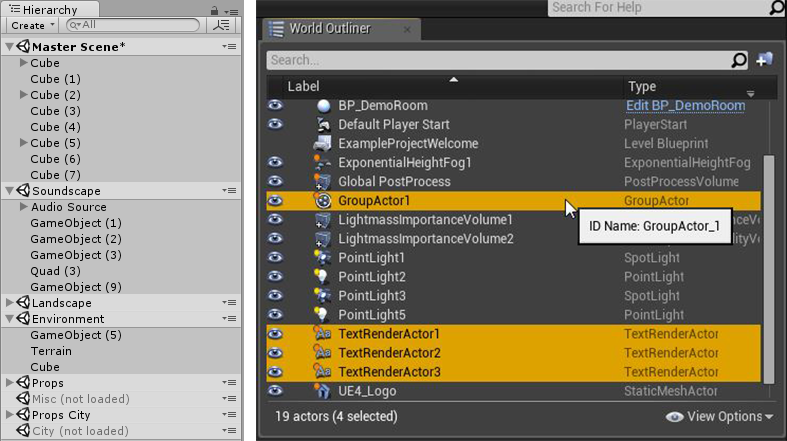
\includegraphics[width=\textwidth]{images/game_engine/scenegraph}
  \caption{Two example game graphs of the Unity3D (left) and the UnrealEngine4
  (right).}
  \label{fig:scenegraph}
\end{figure}

The \textit{Shared Model} concept is mainly inspired by the game graph concept
of game engines. The graph is represented by a \gls{json} document structure and
can be shared either using a Git repository or by using a development database.
The \gls{json} format helps to achieve platform independence.

The \textit{Shared Model} is specifically useful to enable strongly typed
message transfers and unified database access. The design of the \textit{Shared
Model} allows to integrate the game graph into a game engine because the
concepts are closely related.

The \textit{Shared Model} represents the game graph in the form of two
individual trees: the \textit{Template Tree} and the \textit{Prefab Tree}. The
\textit{Template Tree} is responsible for storing types. \textit{Template Types}
are blueprints to define all entities of the game. Entities are not restricted
to one purpose and can be used to store or transmit domain data.
\textit{Template Types} are plain data objects and can be thought of as the
equivalent to Java POJOs. At the moment it is not possible to add game logic to
\textit{Template Types}. But this is planned for the future by using code
injection (explained in \autoref{sub:model_code_injection}).
\autoref{lst:template_type} shows an example of a \textit{Template Type} in the
\textit{Template Tree}.

\begin{figure}
\begin{lstlisting}[language=json,firstnumber=1] 
{
  "name": "UserValues",
  "variables": [
    {
      "name": "id",
      "type": {
        "numberType": "INT",
        "type": "NUMBER"
      }
    },
    {
      "name": "credentials",
      "type": {
        "componentType": "CredentialValues",
        "type": "COMPONENT"
      }
    }
  ]
}
\end{lstlisting}
\caption{The \textit{Template Type} for the UserValues domain object in the \textit{Template Tree}.}
\label{lst:template_type}
\end{figure}

The types supported of the \textit{Template Tree} are directly derived from the
java types because they natively work with the Java side of MicroNet. The Java
types are well documented in the Java language definition and can therefore be
replicated in other programming languages to achieve deterministic behaviour on
all systems.
The supported types are: STRING, NUMBER (INT, FLOAT, DOUBLE, \ldots), BOOLEAN,
CHAR, ENUM, LIST, SET, MAP, and COMPONENT. More information about the supported
types can be found in paragraph on the \textit{Model Editor} in
\autoref{sub:tools}.

The second tree is the \textit{Prefab Tree}. It is responsible for storing
actual instances of \textit{Template Types} representing the statical part of the game
state. The \textit{Prefab Tree} is a concept to allow game designers to define the
properties of the game in a way which is directly understood by MicroNet and
which can therefore be directly used to persist and synchronize the game.
\autoref{lst:prefab_type} shows how a \textit{Prefab} of the \code{UserValues}
object looks like.

\begin{figure}
\begin{lstlisting}[language=json,firstnumber=1] 
{
  "id": 42,
  "credentials": {
    "username": "Jonas",
    "password": "1234"
  }
}
\end{lstlisting}
\caption{A \textit{Prefab} of the UserValues \textit{Template Type}.}
\label{lst:prefab_type}
\end{figure}



\subsubsection{Service API}

The messaging system described in \autoref{sub:networking} is the main driver
for logical composition in MicroNet applications. The \textit{Service API} is
offered to the user by the \gls{api} gateway in the form of a URI addressing. \mss{}
can also use this scheme to find each other internally. The only requirement to
use the \gls{api} is to have access to the underlying message broker either
through the MicroNet networking component or through a direct connection to
ActiveMQ.

The MicroNet \textit{Service API} is defined by using static URIs using the
specific form: \textit{ms://servicename/fine/grained/api}. The host portion of
the URI is used for participant discovery by using the message broker
functionality to register queues at the specific service address,
\textit{ms://servicename} in this example. The remainder of the URI,
\textit{fine/grained/api} in this example represents the fine grained
\textit{Service API} defined by the \ms{} according to tenet of Fine-grained
Interfaces. This \textit{Service API} scheme of MicroNet is inspired by a
RESTful URI schema but is only static\footnote{Requests to URIs like
\textit{mn://player/123341214/some/functionality} are not realized.}. Within
\mss{} the \textit{Service API} is defined using Java annotations described in
the paragraph Annotations in \autoref{sub:tools}.

\subsubsection{Service Catalogue}

The service catalogue is a layer of MicroNet that uses the underlying framework
to provide reference service implementations for commonly required
functionality. The service catalogue is realized by using Maven archetypes. An
archetype represents a skeleton or a basic implementation of a feature and can
be extended by the developer. It is possible for developers to contribute
services to a private service catalogue by creating a new Maven archetype and
making them available for future use. \autoref{fig:service_catalogue} shows
how the service catalogue is integrated into the game development process.

\begin{figure}
	\centering
	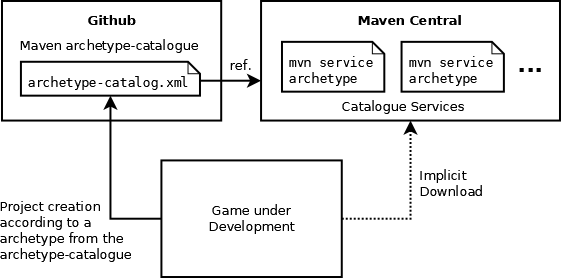
\includegraphics[width=12cm]{images/architecture/ServiceCatalogue}
	\caption{Integration of the service catalogue in \og{} development.}
	\label{fig:service_catalogue}
\end{figure}

The \ms{} mostly used of the service catalogue is the ``Hello World''
service which provides the means of quickly bringing up a new \ms{}. 

\subsubsection{Consistency Requirements}

Consistency is a big concern in any distributed application and \ogs{} are no
exception. Consistency requirements for \ogs{} have already been researched in
project thesis one \cite{biedermann2015project1} in section 5.4 Non-functional
requirements and have been further examined in this semester.

For \ogs{} consistency requirements can be categorized into strong consistency
for sensitive data like account or payment information and eventual consistency
for all other non critical game data. 

The final solution to consistency in MicroNet emphasises exactly these two
requirements. For transactions which require strong consistency it is aways
necessary for one single \ms{} to maintain the overall control over the complete
transaction. This service must then use the underlying relational database to
make the transaction ACID by using the two phase commit protocol offered by the
database which is ProstgreSQL for MicroNet. This approach is mainly chosen due
to the reason that ACID transactions using eventual consistency are hard to get
right and are therefore error-prone \cite{zhang2011transaction},
\cite{zhang2008persistence}, and \cite{pardon2014atomic}.

For game functionality which does not involve financial or sensitive user data
eventual consistency is a solution that has proven to work
\cite{graham2016distributed_transactions}. Eventual consistency emphasizes
scaling and robust systems in general. The drawback is the added effort during
development to implement an eventually consistent application.

Eventual consistency in MicroNet is realized by time-outs and retries. This is
realized by using the persistence system of the message broker in conjunction
with the request response functionality offered by MicroNet messaging. \mss{}
are advised to retry a transaction for a number of times\footnote{Five retries
seemed appropriate for most requests.}. If all retries were failures the service
must persistently log the unprocessed transaction to be either examined either
automatically by a dedicated error handling service or by a developer. In this
error case an informative message to the user. With this approach bugs in the
application which are otherwise difficult to find can be located and fixed which
should decrease the number of unprocessed transactions over time.
